
\chapter{Galois (or Finite) Fields}

In this appendix we introduce some basic coding concepts related to error correction coding with a particular focus on mathematical tools come in useful through DVB-S2 FEC encoding. Obviously, we do not provide a complete treatment of such a rigorous and abstract mathematical theory. First, because it not so worth for our purposes; second, because there are several books written over Coding Theory where is exhaustively and rigorously explained all that could be necessary. Therefore, for any further information over the next presented topics, the reader could refer, for example, to \cite{b:moon} or \cite{b:mcwilliams}.

In engineering application it is often necessary finding a reasonable trade-off between system complexity and performance achieved. On the one hand, elementary decoding approach is simpler, but, on the other hand, its computational burden increases exponentially with the length of code. Algebraic decoding represents a valid alternative to overcome such an huge complexity grow.

The key idea concerning the algebraic coding is that of giving to codes some algebraic structure to be exploited for decoding purposes. When length of block become rather great decoding turn out to be somewhat intractable. For example, the hard decision on the minimum distance between any received sequence and codewords requires an computational effort and a big amount of memory, both increasing with the length of code. An other approach is the \emph{standard array decoding}. Unfortunately, this also turns out to be too expensive when the block dimensions become large. In particular, its memory requirements make this approach rather unattractive.

Algebraic coding/decoding is based on a large extent of powerful and elegant algebraic structures called finite fields.
A field is essentially a set of elements where addition, subtraction, multiplication and division operations yield always an element within such set. A well known example of a field is \(\mathbb R\), the infinite field of real numbers. Although the following observation could be rather trivial, the need of such an algebraic structure is straightforward. Finite fields act as the most common real fields. The unique difference is that the size of the set is finite as, for example, an ensemble of codewords. Note, for example, that any codeword could not be decoded by Berlekamp-Massey algorithm or Galois Field Transform if inverse property was not satisfied.

Although the preliminary concepts over axioms and elementary algebraic structures which lead to rigorous mathematical definition of field properties are even important, the real core of this appendix is the part as to factorization of a `special polynomial'. This operation provides, together with some elementary knowledge on the Coding Theory, a powerful tool to design and well understand algebraic encoding and decoding algorithms.

\section{Algebraic Structures: a Glance} \label{sec:algebraicstruct}
Before discussing properties of finite fields, let us define some preliminary algebraic structures. Let us start from the definition of groups. On this sets it is possible to define some (binary) operations between their elements. To be called a group, operations over such a set must satisfy these following algebraic properties.

\begin{Def}
A binary operation \(\ast\) on a set assigns to each ordered pair of elements of the set $(a\virgola b)$ some element of the set. (This is defined as \emph{closed} binary operation.)
\end{Def}
\begin{Def}
A \emph{group} is a set $\langle G \virgola + \rangle$ together with a binary operation $\ast$ on $G$ such that:
\itemize
\item[G1] The operator is \emph{associative}: for any \(a \virgola b \virgola c \in G \virgola (a \ast b)\ast c= a \ast (b \ast c).\)
\item[G2] There is an element \(e \in G\) called the \emph{identity element} such that \( a\ast e = e \ast a \) for all \( a \in G\).
\item[G3] For every \( a \in G\), there is an element \(b \in G\) known as the \emph{inverse} of $a$ such that \(a \ast b = e\) The inverse of a is sometimes denotes as \(a^{-1}\) (when the operator $\ast$ is multiplication-like) or as $-a$ (when the operator $\ast$ is addition-like).
\item[G4] If also \( a \ast b  \) is equal to \(b \ast a\), the group is also an abelian (or commutative) group.
\end{Def}
If the commutative property holds then a group is said abelian. It is possible to define an algebraic structure as a group also on a finite set of elements, as well as on those infinite.

\begin{Def}
If $G$ has a finite number of elements, it is said to be a finite group. Furthermore, such number is called the order (or the cardinality) of the group.
\end{Def}

Let \( \langle \mathbb Z_n \virgola + \rangle \) denote addition on the numbers \( \{0 \virgola 1 \virgola \ldots \virgola n-1 \}\) modulo $n$. Clearly such set is an abelian group, since, as it is shown in explicative Table \ref{tb:Ringmod6} (which can be easily generalized) 0 is the identity element appearing in each column; moreover, the uniqueness of solution proves associative property; furthermore, the addition table or its generalization is symmetric and thus the operation is commutative.

%Let us consider a source that transmits symbols from an alphabet $\mathcal A$ having $q$ symbols, where $\mathcal A$ forms a \emph{field}. We refer to a tuple \( (c_0 \virgola c_1 \virgola \ldots \virgola c_{n-1}) \in \mathcal A^n \) with $n$ elements as an $n$-vector or an $n$-tuple. %
Let us now introduce another algebraic structure, the \emph{ring}, which will be later helpful in the examination of cyclic codes. Differently from groups, \emph{rings} have two binary operation associated with them.
\begin{Def}
A \emph{ring} (loosely speaking) is a set where addition, subtraction and multiplication are possible. Formally, \(R\) is an additive abelian group, together with a multiplication satisfying \(ab=ba\), \(a(b+c)=ab+ac\), \((ab)c = a(bc)\), and which contains an identity element 1 such that \(1\cdot a=a\).
\end{Def}
As also shown in Table \ref{tb:Ringmod6}, the multiplication under \( \mathbb Z_{n}\) does not form a group: there is a presence of zeros in correspondence of columns which denote the nonzero elements (see the next section for the \emph{zero divisor} formal definition). In fact, in a ring, not every element has a multiplicative inverse, whereas, in a \emph{field}, the familiar arithmetic operations that take place in the usual real numbers are all available.

\begin{Def}
A \emph{field} is a set of objects \( \mathbb F\) on which the operations of addition and multiplication, subtraction (or additive inverse), and division (or multiplicative inverse) apply in a manner analogous to the way these operation work for real numbers. That is
\itemize
\item[F1]  The elements of \( \mathbb F \) form an abelian (or commutative) \emph{group} under addition.
\item[F2] The non-zero elements of \( \mathbb F\) form an abelian \emph{group} under multiplication.
\end{Def}

\begin{table}\centering
\begin{tabular}{c| c c c c c}
+ & 0 & 1 & 2 & 3 & 4\\
\hline
0 & 0 & 1 & 2 & 3 & 4\\
1 & 1 & 2 & 3 & 4 & 0\\
2 & 2 & 3 & 4 & 0 & 1\\
3 & 3 & 4 & 0 & 1 & 2\\
4 & 4 & 0 & 1 & 2 & 3\\
\end{tabular}
\caption{Addition table under \( \mathbb Z_5\)\label{tb:Rmod5}}
\end{table}

\begin{table}\centering
\begin{tabular}{c| c c c c c c}
$\cdot$ & 0 & 1 & 2 & 3 & 4 & 5\\
\hline
0 & 0 & 0 & 0 & 0 & 0 & 0\\
1 & 0 & 1 & 2 & 3 & 4 & 5\\
2 & 0 & 2 & 4 & 0 & 2 & 4\\
3 & 0 & 3 & 0 & 3 & 0 & 3\\
4 & 0 & 4 & 2 & 0 & 4 & 2\\
5 & 0 & 5 & 4 & 3 & 2 & 1\\
\end{tabular}
\caption{Multiplication table under \( \mathbb Z_6\) \label{tb:Ringmod6}}
\end{table}


\section{How Do We Get Galois Fields?} \label{sec:GF}

Let us now try to find a relationship between groups and fields. More specifically, starting from the rings with addition and multiplication operations modulo $n$, we wish to comprehend how obtaining a finite field and under which hypothesis.
To this purpose, it could be interesting to note that, in some cases, each nonzero element of a ring has a multiplicative inverse and so is a field, while, in other ones, there exist some elements without a multiplicative inverse. We could start to observe that when the ring characteristic is a prime number (as five, see Table \ref{tb:Fieldmod5}), we have a ring with elements forming an abelian group under multiplications. The reasons will be made more clear after this following definition as to elements called as zero divisors.

\begin{Def}
In a ring $R$, if \(a \virgola b \in R\) with both $a$ and $b$ not equal to zero but \(ab = 0\), then $a$ and $b$ are said to be \emph{zero divisors}.
\end{Def}
In practice, the presence of zero divisors make a ring impossible to have a multiplicative inverse for each its elements and, above all, have a multiplicative structure closed under multiplicative operations.Therefore, if we have no zero divisors then a finite ring is also a Galois (or finite) field. The following theorem defines under which hypothesis no such elements exist.

\begin{Theorem}[Todd K.~Moon, \cite{b:moon}]
The ring \( \mathbb Z_p\) is a field if and only if p is a prime.   \label{th:subgf}
\end{Theorem}
Without making any mathematical calculations, we can observe (as proof) that if $p$ is a prime its multiples over \( \mathbb Z_p\) cannot exist and, therefore, neither zero divisors.

Besides the finite fields with $p$ prime, there are other finite fields. As the field of complex numbers \( \mathbb C\) can be constructed as a field extension from the field of real numbers \(\mathbb R\), these Galois fields are \emph{extension fields} of \( \mathbb Z_p\). More in detail, extension fields are constructed to create roots of irreducible polynomials that do not have roots in base fields. E.g., the  polynomial \(f(x) = x^2+1\) is irreducible over \(\mathbb R\), but not over \(\mathbb C\) where we can write:
\begin{equation}
f(x)=(x+\alpha)(x-\alpha)=(x+\im)(x-\im)
\end{equation}
Practically we obtain an extension field from a base field whenever we can find any irreducible polynomial over the base field. Loosely speaking, these polynomials may be conceived as prime numbers by which (as noticed previously) it is possible to construct any fields.

\begin{table}\centering
\begin{tabular}{c| c c c c c}
$\cdot$ & 0 & 1 & 2 & 3 & 4\\
\hline
0 & 0 & 0 & 0 & 0 & 0\\
1 & 0 & 1 & 2 & 3 & 4\\
2 & 0 & 2 & 4 & 1 & 3\\
3 & 0 & 3 & 1 & 4 & 2\\
4 & 0 & 4 & 3 & 2 & 1 \\
\end{tabular}
\caption{Multiplication table under \( \mathbb Z_5\)} \label{tb:Fieldmod5}
\end{table}


\section{A Mathematical Survey} \label{sec:MathSurvey}
Having shown how to obtain Galois fields, we now lay out some aspects of the theory. We first focus on the additive structure of finite fields, which tells us what size any finite fields can be. Recalling Theorem \ref{th:subgf}, it follows that there are $p$ elements which behave as a field (i.e., we can define addition and multiplication on them as a field). Thus, \( \mathbb Z_p\) is a subfield of every Galois fields $GF(q)$. In fact, an assertion can be made:

\begin{Theorem}[Todd K.~Moon, \cite{b:moon}]
The order $q$ of every finite fields $GF(q)$ must be a power of a prime.
\end{Theorem}

By Theorem~\ref{th:subgf}, every finite fields $GF(q)$ has a subfield of prime order $p$. In fact, it can be shown that $GF(q)$ acts like a vector space over its subfield $GF(p)$. More specifically, if we get
\begin{equation}
a_1\beta_1 + a_2\beta_2 + \ldots + a_m\beta_m
\end{equation}
with coefficients \(a_i\) lying over $GF(p)$ and $\beta_i \in GF(q=p^m)$ we can obtain all the distinct elements of $GF(q)$. In other words, each combination of coefficients \( \{a_1 \virgola a_2 \virgola \cdots \virgola a_m\}\) corresponds to a distinct element of $GF(q)$.

This theorem shows that all finite fields have the structure of a vector space of dimension $m$ over a finite field \( \mathbb Z_p\). For the field $GF(p^m)$, the subfield $GF(p)$ is called the \emph{ground field}.

By definition, each element of a finite field forms a group under multiplication. Let us now try to understand how they behave, giving at the same time some helpful definitions.

\begin{Def}
Let $\beta \in GF(q)$. The \emph{order}  \footnote{The nomenclature is slightly misguiding, since we already defined the order of a group.}
 of $\beta$, written ord($\beta$) is the smallest positive integer such that \(\beta^n=1\).
\end{Def}


\begin{Def}
An element with order $q-1$ in $GF(q)$ (i.e, it generates all the nonzero elements of the field) is called \emph{primitive element}.
\end{Def}

In other words, a primitive element has the highest possible order. Since every elements of the field are representable by that, this `special element' (or elements) enables the `power representation' of the field, which much simplify multiplication.
In the brackets of this last sentence we have referred to a more than one possible existence of these primitive elements. More specifically, they are \( \phi(q-1) \) (i.e., Euler totient function \cite{b:moon}), as following theorem asserts.


\begin{Theorem}[Todd K.~Moon, \cite{b:moon}]
There are $\phi(q-1)$ primitive elements in $GF(q)$.
\end{Theorem}

If \(\alpha \in GF(q)\) is primitive, then
\[
\{\alpha \virgola \alpha^2 \virgola \ldots \virgola \alpha^{q-2} \virgola \alpha^{q-1}=1 \}
\]
is the set of nonzero elements of \(GF(q)\). But, if \(\beta=\alpha^i\) is also primitive then the nonzero elements of the fields are still generated by
\[
\{\beta \virgola \beta^2 \virgola \ldots \virgola \beta^{q-2} \virgola \beta^{q-1}=1 \}
\]
Although these are different generators, these are not different fields, but only different representations.

Since, as we previously said, every field element can be written as \(\beta=\alpha^i \in GF(q) \) we have the following.

\begin{Theorem}[Todd K.~Moon, \cite{b:moon}]
Every element of the field $GF(q)$ satisfies the equation \(x^q-x=0\). Furthermore, they constitute the entire set of roots of this equation. \label{th:roots}
\end{Theorem}
Its proof is trivial: let $\alpha$ a primitive element. Then imposing \(\beta = \alpha^i \) yields \( {(\alpha^i)}^{q-1} = {(\alpha^{q-1})}^{i} =1 \) which satisfies the equivalent equation \(x^{q-1}-1=0\).
\label{th:FieldGFBuild}


\section{Irreducible and Primitive polynomials} \label{sec:primpoly}

While any irreducible polynomial can be used to construct the extension field, computation in the field is easier if a primitive polynomial is used. We make the following observation:

\begin{Theorem}[Todd K.~Moon, \cite{b:moon}]
Let $p$ a prime. An irreducible mth-degree polynomial $f(x) \in GF(p)[x] $ divides \( x^{p^m-1}-1\).
\end{Theorem}

Let \(GF(q)=GF(p^m) \) be constructed using the irreducible polynomial \(f(x)\), where \(\alpha\) denotes the root of \(f(x)\) in the field: \(f(\alpha)= 0\). By Theorem~\ref{th:roots}, $\alpha$ is a root of \(x^{p^m-1}-1\) in \(GF(q)\). Using the division algorithm (i.e., Euclid theorem) write
\begin{equation}
x^{p^m-1}-1= g(x)f(x)+r(x)
\end{equation}
where \( \mathrm{deg}(r(x)) \le m\). Evaluating above equation at \(x=\alpha\) we obtain
\[
0 = 0 + r(\alpha)
\]
But the elements of the field \(GF(q)\) are represented as polynomials in $\alpha$ of degree less equal to \(m\), so since \(r(\alpha)= 0\) it must be that \(r(x)\) is a zero polynomial, \(r(x) = 0\).

\begin{Def}
An irreducible polynomial \(p(x) \in GF(p)[x] \) of degree \(m\) is said to be \emph{primitive} if the smallest positive integer \(n\) for which \(p(x)\) divides \(x^n-1\) is \(n=p^m-1\).
\end{Def}

\begin{Theorem}[Todd K.~Moon, \cite{b:moon}]
The roots of an mth degree primitive polynomial \( p(x) \in GF(p)[x] \) are primitive elements in \(GF(p^m)\)
\end{Theorem}
In other words, any of the roots can be used to generate the nonzero elements of the field \(GF(p^m)\). Furthermore, all the nonzero elements of the field can be generated as power of the roots of the primitive polynomial.

\section{Factoring $x^n-1$ } \label{sec:factoring}

To design and understand cyclic codes, it is worth succeeding in factorization of \(x^n-1\) over arbitrary finite fields.

From Theorem~\ref{th:roots}, we know that every element of \(GF(q^m) \) is a root of \(x^{q^m-1}-1\), so \[
x^{q^m-1}-1= \prod_{i=0}^{q^m-1} {(x-\alpha^i)}
\]
for a primitive element \( \alpha \in GF(q^m) \). To provide a factorization over the field \(GF(q)\) , the factors \(x-\alpha^i\) can be grouped together according to conjugacy classes. First of all, let us describe some concepts related to.

\begin{Def}
Let $\beta \in GF(q^m)$. The \emph{conjugates} of \(\beta\) with respect to a subfield \(GF(q)\) are \( \beta \virgola \beta^q \virgola \beta^{q^2} \virgola \beta^{q^3} \virgola .... \).
\end{Def}
Since the field is finite, the above list must repeat at some point. This is provided by the following.
\begin{Def}
The smallest positive integer \(d\) such that n is divisible by \(q^d-1\) is called \emph{multiplicative order of \(q\) modulo \(n\)}.
\end{Def}
Furthermore, if any \(\beta \in GF(q^m)\) have \( \mathrm{ord}(\beta)=n\) and \(d\) multiplicative order of \(q\) modulo \(n\), then \(\beta^{q^d} = \beta\). The \(d\) elements
\( \beta \virgola \beta^q \virgola \beta^{q^2}  \virgola \ldots \virgola \beta^{q^{d-1}} \)
are all distinct. In addition, it can be proved the following.

\begin{Theorem} [Todd K.~Moon, \cite{b:moon}]
Let \(\beta \in GF(q^m) \) have order \(n\) and let \(d\) be the multiplicative order of \(q\) mod \(n\). Then the coefficients of the polynomial
\(p(x)=\prod_{i=0}^{d-1}{(x-\beta^{q^i})} \)
are in $GF(q)$. Furthermore, $p(x)$ is irreducible. That is, \(p(x)\) is the minimal polynomial for \(\beta\).
\end{Theorem}

\begin{table}\centering
\begin{tabular}{c| c}
Conjugacy Class & Minimal Polynomial\\
\hline
\(\{ 0\}\) & \(x\) \\
\(\{ 1\}\) & \(x+1\) \\
\(\{ \alpha \virgola \alpha^2 \virgola \alpha^4 \}\) &
\( (x-\alpha)(x-\alpha^2)(x-\alpha^4)= x^3+x+1 \) \\
\(\{ \alpha^3 \virgola \alpha^6 \virgola \alpha^5 \}\) &
\( (x-\alpha^3)(x-\alpha^6)(x-\alpha^5)= x^3+x^2+1 \)
\end{tabular}
\caption{ Conjugacy Classes over \(GF(2^3)\) with respect to \(GF(2)\) \label{tb:MinPoly3}}
\end{table}

\begin{table}\centering
\begin{tabular}{c| c}
Conjugacy Class & Minimal Polynomial\\
\hline
\(\{ 0\}\) & \(x\) \\
\(\{ 1\}\) & \(x+1\) \\
\(\{ \alpha \virgola \alpha^2 \virgola \alpha^4 \virgola \alpha^8\}\) &
\( (x-\alpha)(x-\alpha^2)(x-\alpha^4)(x-\alpha^8)= x^4+x+1 \) \\
\(\{ \alpha^3 \virgola \alpha^6 \virgola \alpha^9 \virgola \alpha^{12} \}\) &
\( (x-\alpha^3)(x-\alpha^6)(x-\alpha^9)(x-\alpha^{12})= x^4+x^3+x^2+x+1 \) \\
\(\{ \alpha^5 \virgola \alpha^{10}\}\) &
\( (x-\alpha^5)(x-\alpha^{10})= x^2+x+1 \) \\
\(\{ \alpha^7 \virgola \alpha^{11} \virgola \alpha^{13} \virgola \alpha^{14}\}\) &
\( (x-\alpha^7)(x-\alpha^{11})(x-\alpha^{13})(x-\alpha^{14})= x^4+x^3+1 \)
\end{tabular}
\caption{ Conjugacy Classes over \(GF(2^4)\) with respect to \(GF(2)\) \label{tb:MinPoly4}}
\end{table}

We now are ready to understand that \(x^{q^m-1}-1\) can be expressed as a product of the minimal polynomials of the nonzero elements. For example the polynomial
\(x^7-1 = x^{2^3-1}-1\)
can be factored over \(GF(2)\) as a product of the minimal polynomials shown in Table~\ref{tb:MinPoly3}
\begin{equation}
x^7-1=(x+1)(x^3+x+1)(x^3+x^2+1)
\end{equation}

To generalize problem of factoring \(x^n-1\) when \(n \ne q^m-1\), let any element \(\beta \ne 1\) such that \(\beta^n = 1\) call a \(n\)th root of unity. First, we have to determine a field \(GF(q^m)\) where \(n\)th root of unity can exist. Once found, factorization is accomplished using the minimal polynomials in such field.

Since there are \( \phi(n)\) elements of order \(n\) in \(GF(q^m)\), finding a field \(GF(q^m)\) with \(n\) roots of unity requires finding an \(m\) such that \(n|q^m-1\) (i.e, \(n\) must be a divisor of \(q^m-1\)). This is usually done by trial and error.

Once any \(\beta\) of order \(n\) is found, then \(beta\) is a root of \(x^n-1\) in that field, and so are the elements \(\beta^2 \virgola \beta^3 \virgola \ldots \virgola \beta^{n-1} \). In other words,
\begin{equation}
x^n-1= \prod_{i=0}^{n-1}{x-\beta^i}
\end{equation}

For example, let now determine an extension field \(GF(2^m)\) in which 5th roots of unity exist and express the factorization in term of polynomials in \(GF(2)[x]\). Since 5 is the smallest divisors of \(2^4-1\), the roots of unity are over \(GF(16)\). So if we let \(\beta=\alpha^3\), \(\alpha\) primitive, then \(\beta^5=\alpha^15=1\). Thus the roots of \(x^5-1=x^5+1\) in \(GF(16)\) are
\[
1 \virgola \beta \virgola \beta^2 \virgola \beta^3 \virgola \beta^4
\]
which can be expressed in terms of the primitive element \(\alpha\) as
\[
1 \virgola \alpha^3 \virgola \alpha^6 \virgola \alpha^9 \virgola \alpha^{12}
\]
Using the minimal polynomials shown in Table~\ref{tb:MinPoly4} we have
\[
x^5-1=(x+1)(x^4+x^3+x^2+x+1)
\]

\chapter{Cyclic Codes}

We now deal with \emph{cyclic codes}, which have additional algebraic structure to make encoding and decoding more efficient. In other words, they have some structure that can be easily exploited through encoding/decoding stages. Note that one of the most notorious cyclic codes are the Hamming codes. In fact, from a certain point of view, BCH codes can be conceived as an extension of Hamming codes. This `parallelism' is well shown in \cite{b:wicker}, \cite{b:mcwilliams}.

Cyclic codes are based on polynomial operations. A natural algebraic settings for the operation on polynomials is the algebraic structure of a ring.
This appendix presents some elementary concepts related to shift operations and linear block codes, focusing on the algebraic description of cyclic codes. Galois fields and cyclic codes theory together are exploited in the design of a cyclic code with a specified minimum distance. The theoretical and practical connection between algebraic structures and code description shows a way of reducing the computational burden in decoding.

\section{Shift Operation} \label{sec:shift}
We now introduce the mathematical definition of cyclic block codes.
\begin{Def}
A \( (n \virgola k) \) block code $\mathcal C$ is said to be cyclic if it is linear and if for every codeword \( \vet{c}=(c_0 \virgola c_1 \virgola \ldots \virgola c_{n-1}) \) in $\mathcal C$, its right cyclic shift \( \vet{c'}=(c_{n-1} \virgola c_0 \virgola \ldots \virgola c_{n-2}) \) is also in \( \mathcal C \).
\end{Def}

The operations of shifting and cyclic shifting can be conveniently represented using polynomials. The vector
\begin{equation}
 \vet{c}=(c_0 \virgola c_1 \virgola \ldots \virgola c_{n-1})
\end{equation}
is represented by the polynomial
\begin{equation}
c(x) = c_0 + c_1x+\ldots+c_{n-1}x^{n-1}
\end{equation}
using the obvious one-to-one correspondence.
A (noncyclic) shift can be represented by polynomial multiplication:
\begin{equation}
xc(x)= c_0x + c_1x^2+\ldots+c_{n-1}x^{n}
\end{equation}
However, if c(x) was a hypothetic codeword, the above operation obviously would not yield any codeword.

As described in Appendix A, taking the remainder after division by \(x^n-1\) translates into imposing \(x^n=1\). So that getting \(xc(x) \) module \(x^n-1\) yields
\begin{equation}
xc(x)=c_{n-1} + c_0x + c_1x^2+\ldots+ c_{n-2}x^{n-1}
\end{equation}
Could this result be any codeword, or rather, any element of the same set? In other words, this point is that mathematicians call closure under a given operation (or operator).
Before dealing with this, we need to introduce another algebraic structure, the \emph{ideals}. It will show that every cyclic codes forms ideals in a \emph{ring of polynomials}.



\section{Rings of Polynomials and Ideals in Rings} \label{sec:ideals}

Let $R$ be a ring. A polynomial \( f(x) \) of degree $n$ with coefficients in $R$ is
\begin{equation}
f(x) = \sum^{n}_{i=0}{a_ix^i}
\end{equation}
where \( a_n \neq 0 \). The symbol $x$ is said an \emph{indeterminate}.

\begin{Def}
The set of all polynomials with an indeterminate $x$ with coefficients in a ring $R$, using the usual operations for polynomial addition and multiplication, forms a ring called the \emph{polynomial ring}. It is denoted as $R[x]$.
\end{Def}
Generally, polynomial multiplication has not an inverse. For example in the ring of polynomials with real coefficients $\mathbb R [x]$, there is no polynomial solutions $f(x)$ to
\[
f(x)(x^2+5x+1) = x^3+3x+1
\]

Let us now consider the residue class of polynomials rings \( GF(p)[x] \) modulo \(x^n-1\), denoted as \(GF(p)[x]/(x^n-1)\). We have already shown (\ref{sec:GF}) that a quotient ring is a field if and only if \(x^n-1\) cannot be factored over the base field \(GF(p)\) ($p$ is a prime number).
But let us return to our main question. In fact, we would like to find a set where every its shifted elements is still within such set. Such an algebraic structure is the following.

\begin{Def}
Let $R$ be a ring. A nonempty subset $I\subseteq R$ is an \emph{ideal} if satisfies the following conditions:
\begin{enumerate}
\item $I$ forms a group under the addition operation in $R$.
\item For any \( a\in I\) and any \(r\in R\), \(ar\in I\).
\end{enumerate}
\end{Def}
It seems that a cyclic code form an ideal in a ring of polynomials. Furthermore, for cyclic codes the ideals are principal, as defined by the following.

\begin{Def}
An ideal $I$ in a ring $R$ is said to be \emph{principal} if there exist some \(g\in I\) such that every element \(a \in I \) can be expressed as a product \(a=mg\) for some \(m \in R\).For a principal ideal, such an element \(g\) is called the \emph{generator element}. The ideal generated by \(g\) is denoted as \(\langle g \rangle\):
\[
\langle g \rangle= \{hg: h \in R \}
\]
\end{Def}

\begin{Theorem}[Todd K.~Moon, \cite{b:moon}] \label{th:ideals}
Let $I$ be an ideal in \( \mathbb F_q /(x^n-1) \). Then
\enumerate
\item There is a unique monic polynomial \(g(x) \in I\) of minimal degree.
\item $I$ is principal with generator $g(x)$.
\item \(g(x)\) divides \( (x^n -1) \) in \( \mathbb F_q[x] \).
\end{Theorem}
For example, it can be shown that in \(GF(2)[x]\)
\[
x^7-1=(x+1)(x^3+x+1)(x^3+x^2+1)
\]
In the ring \( GF(2)[x]/(x^7-1) \), there are ideals corresponding to the different factorization of \(x^7+1 \virgola\) so there are the following nontrivial ideals
\begin{alignat*}3
     & \langle x+1 \rangle & \qquad \langle x^3+x+1\rangle & \qquad \langle x^3+x^2+1\rangle \\
     & \langle (x+1)(x^3+x+1)\rangle & \qquad \langle (x+1)(x^3+x^2+1)\rangle & \qquad
     \langle (x^3+x^2+1)(x^3+x+1)\rangle
\end{alignat*}

\section{Algebraic Description}

As said in Section~\ref{sec:shift}, cyclic shifting of a polynomial \(c(x)\) is represented by \(xc(x)\) modulo \(x^n-1\) operation. Taking into account Theorem \ref{th:ideals} and what said as far, we can therefore reach the following conclusions as to cyclic codes:
\begin{itemize}
\item A $(n \virgola k)$ cyclic code has a unique minimal monic polynomial
\begin{equation}
    g(x) = g_0+g_1x+\ldots+g_{n-k}x^{n-k}
\end{equation}
It, which is also the generator of ideal, is called the \emph{generator polynomial} for the code, and its degree represents the redundancy $r=n-k$ of the code.

\item Every codeword can be expressed as a multiple of the generator
\begin{equation}
c(x)=m(x)g(x)
\end{equation}
Obviously, the degree of message polynomial $m(x)$ is less than $k$, so the dimension of the code is $k$. In other words, there are $k$ independently selectable coefficients in $m(x)$.

Generalization for the systematic coding is straightforward. In fact, by Euclid Theorem application we have
\begin{equation}
m(x)x^{n-k}= q(x)g(x)+r(x) \Rightarrow m(x)x^{n-k}-r(x) = q(x)g(x)
\end{equation}
and therefore if we conceive a codeword as $m(x)x^{n-k}-r(x)$ where $r(x)$ represents the remainder of $m(x)$ after division by $g(x)$, then we obtain an equivalent representation of cyclic code. This is called in literature systematic form and it has the following vector correspondence
\begin{equation}
(-d_0\virgola -d_1\virgola \ldots \virgola -d_{n-k-1}\virgola m_0 \virgola m_1 \virgola \ldots \virgola m_{k-1}) \leftrightarrow x^{n-k}m(x)-r(x)
\end{equation}
Loosely speaking, this different encoding process has the unique effect of changing one-to-one mapping between messages and correspondent codewords.
\item Furthermore, the generator $g(x)$ is a factor of $x^{n-1}-1$ in $GF(q)[x]$.
\end{itemize}


%\begin{figure}
%\centerline{\psfig{figure=polydiv1.eps,width=12.5cm}}
%\end{figure}

%\begin{figure} \centering
%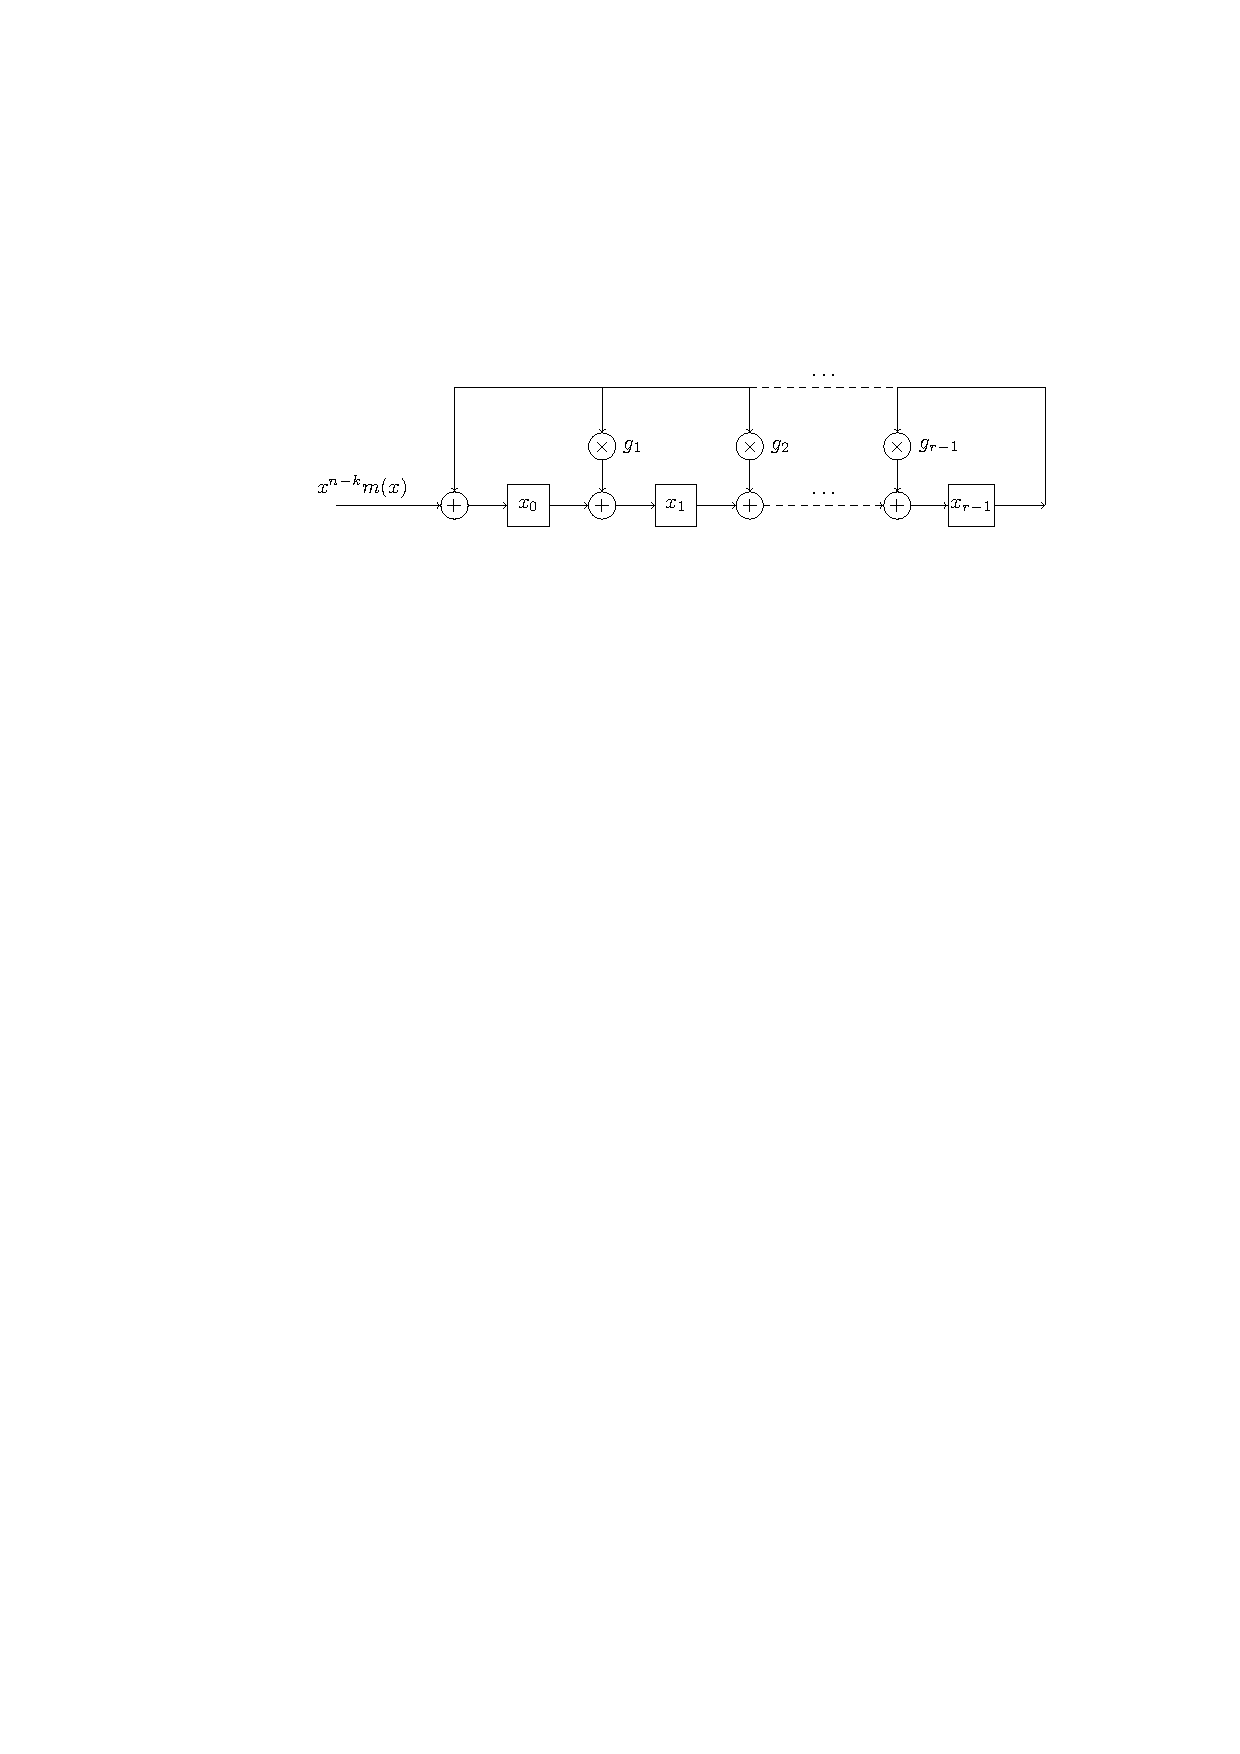
\includegraphics[scale=0.6]{polydiv1}
%\end{figure}

